\section{Глава 2. Методы машинного обучения с учителем}

В данной главе будут рассмотрены методы машинного обучения, используемые в работе, дана краткая характеристика задач, для которых эти методы используются, а также получены результаты по поставленным задачам.

\subsection{2.1. Виды машинного обучения с учителем}
Как правило, выделяют несколько видов машинного обучения с учителем. В данной работе используются:
\begin{enumerate}
\item Классификация. При решении задачи классификации предполагается, что имеется множество объектов разделенных некоторым образом на классы и, при этом, количество классов известно заранее.
\item Регрессия. В задаче регрессии требуется по заданному набору признаков объекта спрогнозировать целевую переменную, которая, как правило, может принимать любое вещественное значение.
\end{enumerate}

\subsection{2.2. Метрики качества}

В данной работе для оценки качества определения возраста используется средняя абсолютная ошибка, которая определяется следующим образом:

$$
	MAE = \frac{\sum_{i=1}^{n} |y_i - \hat{y_i}|}{n}
$$

где $y_i$ - точное значение, $\hat{y_i}$ - предсказанное значение

Для оценки качества классификации в задаче определения пола используются метрики Accuracy, Precision, Recall и F1, которая является гармоническим среднем Precision и Recall. Более формально эти величины определяются следующим образом:

$$
 Accuracy= \frac{T_p + T_n}{T_p + F_p + F_n + T_n}
$$

$$
 Precision = \frac{T_p}{T_p + F_p}
$$
$$
Recall = \frac{T_p}{T_p + F_n}
$$
$$
	F1 = 2 \cdot \frac{Precision \cdot Recall}{Precision + Recall}
$$
где 

$T_p$ (true positives) -- количество объектов которым модель присвоила первый класс и они на самом деле принадлежат первому классу; 

$F_p$ (false positives) -- количество объектов, которые классификатор отнес к первому классу, но  принадлежащие второму классу;

$F_n$ (false negatives) -- количество объектов, которые классификатор отнес ко второму классу, но принадлежащие первому классу;

$T_n$ (true negatives) -- количество объектов которым модель присвоила второй класс и они действительно принадлежат второму классу.

 
 Recall показывает способность алгоритма обнаруживать данный класс, а Precision --  демонстрирует способность отличать этот класс от других. Accuracy же является просто долей правильно классифицируемых объектов.
 

\subsection{2.3. Линейная регрессия}

Линейная регрессия \cite{linear regression} -- это линейная модель, которая устанавливает связь между зависимой переменной $y \in \mathbb{R}$ и одной или несколькими независимыми переменными $x \in \mathbb{R}^d$. Формально данная модель определяется следующим образом:
$$f(x)=w_0 + \sum_{j=1}^{d}x^j w_j$$
$x = (x^1, x^2, ..., x^d)$ -- входной вектор признаков \\
$w = (w_0, w_1, ... ,w_d)$ -- параметры модели

В задаче машинного обучения с учителем мы как правило имеем набор тренировочных данных $(x_1, y_1) ... (x_l,  y_l)$ с помощью которых мы оцениваем неизвестные параметры модели $w$. Самый популярный метод оценки неизвестных параметров модели линейной регрессии -- это метод наименьших квадратов, суть которого состоит в том, чтобы подобрать неизвестные параметры модели $w$ так, чтобы минимизировать функционал ошибки, который представляет собой среднеквадратичную ошибку алгоритма:

\begin{equation}\label{linreg functional}
Q(f, x) = \frac{1}{l}\sum_{i=1}^{l} (f(x_i) - y_i)
\end{equation}

Минимизация данного функционала происходит с помощью оптимизационного подхода, а именно -- метода градиентного спуска.

К преимуществам линейной регрессии можно отнести то, что она хорошо работает на больших объемах данных и на большом числе признаков. Однако существенным недостатком  является то, что качество работы алгоритма может быть низким, если зависимость целевого значения от признаков нелинейная. 

Для решения задачи определения возраста пользователя используется библиотека scikit learn \cite{sklearn}, которая имеет в своем составе уже различные реализации метода линейной регрессии, такие как Ridge, Lasso и ElasticNet. Данные 3 метода являются модификацией исходной модели линейной регрессии, к которой добавляются соответственно L1, L2 и комбинация L1 и L2 регуляризации. Добавление регуляризации помогает при борьбе с переобучением.

Для автоматизации подбора параметров регуляризации из пакета scikit learn используется класс GridSearchCV с кросс-валидацией на 5 частей.

Полученные результаты определения возраста продемонстрированы в Таблице \ref{linreg age table}.

\setlength\extrarowheight{8pt}
\begin{table}[h!]
\begin{tabular}{|c|m{5em}|m{5em}|m{5em}|l|}
\hline
\textbf{Выборка}                                                             & Исходная & Scaled  & OHE    & OHE + Scaled \\ [3ex] \hline  
\textbf{MAE}                                                                 & 5.4882   & 5.4871  & 3.6179 & 3.6127       \\ [2ex] \hline
\textbf{Регуляризация}                                                       & Ridge    & Ridge   & Ridge  & Ridge        \\ [2ex] \hline
\textbf{\begin{tabular}[c]{@{}c@{}}Коэффициент\\ регуляризации\end{tabular}} & 6.251    & 323.746 & 0.001  & 0.001        \\ [3ex] \hline
\end{tabular}
\caption{Результаты линейной регрессии для определения возраста}
\label{linreg age table}
\end{table}

Как видно из Таблицы \ref{linreg age table}, лучше всего себя показала Ridge регрессия на масштабированной выборки с OHE преобразованием. Ridge регрессия заключается в том, что к оптимизированному функционалу (\ref{linreg functional}) добавляется штраф -- L2 регуляризатор, штрафующий модель за слишком большие веса, которые свидетельствуют о переобучении. В итоге задача оптимизации сводится к следующему виду:


$$
Q(f, x) = \frac{1}{l}\sum_{i=1}^{l} (f(x_i) - y_i) + \lambda||w||_2
$$


\subsection{2.4. Логистическая регрессия}
Логистическая регрессия \cite{ESLII} -- это метод классификации, который позволяет прогнозировать апостериорные вероятности принадлежности объектов к классам с помощью линейной разделяющей гиперплоскости. 

Для того, чтобы оценивать апостериорные вероятности вводят так называемое отношение шансов, которое представляет из себя в случае бинарной классификации отношение вероятности принадлежности объекта $x$ к классу 1 ($P(G=1|x)$) к вероятности принадлежности объекта $x$ к классу 0 ($P(G=0|x)$). Логарифм данного отношения пытаются приблизить с помощью линейной функции

\begin{equation}\label{log_reg_eq}
\log \frac{P(G=1|x)}{1 - P(G=1|x)} = w_0 + \sum_{j=1}^{d}x^j w_j
\end{equation}
Делая некоторые преобразования в формуле  (\ref{log_reg_eq}) можно получить апостериорную оценку вероятности

$$P(G=1|x) = \frac{1}{1 + e^{-z}}$$
где $z = w_0 + \sum_{j=1}^{d}x^j w_j$

Параметры модели $w = (w_0, w_1, ... ,w_d)$ подбираются с помощью метода максимального правдоподобия.

Логистическая регрессия, как и любая другая линейная модель, обладает теми же преимуществами и недостатками, а именно: эффективная работа на больших объемах данных и низкое качество на нелинейных зависимостях. 

В данной работе логистическая регрессия используется для оценки пола пользователя социальной сети. Данный метод находится в модуле linear\_models пакета scikit learn.  Результаты, полученные этим методом к задаче определения пола можно наблюдать в Таблице \ref{logreg gender table}.

\setlength\extrarowheight{8pt}
\begin{table}[h!]
\centering
\begin{tabular}{|c|l|l|l|l|}
\hline
\textbf{Выборка}                                                           & Исходная & Scaled & OHE   & OHE + Scaled \\ \hline
\textbf{Accuracy}                                                          & 0.69     & 0.685  & 0.71  & 0.7          \\ \hline
\textbf{Precision}                                                         & 0.66     & 0.5  & 0.77  & 0.636       \\ \hline
\textbf{Recall}                                                            &  0.0317     & 0.317   & 0.11  & 0.11         \\ \hline
\textbf{F1}                                                                & 0.061     & 0.059   & 0.194 & 0.189         \\ \hline
\textbf{Регуляризация}                                                     & L1       & L1     & L1    & L2           \\ \hline
\textbf{\begin{tabular}[c]{@{}c@{}}Коэффициент \\ регуляризации\end{tabular}} & 0.0336   & 0.234  & 0.234 & 3792.69      \\ \hline
\end{tabular}
\caption{Результаты логистической регрессии для определения пола}
\label{logreg gender table}
\end{table}

Как видно из таблицы данный метод имеет приемлемое значение по метрикам Accuracy и Precision, однако по метрикам Recall и F1 наблюдается низкое качество по всем выборкам. 

\subsection{2.5. Метод опорных векторов}
Метод опорных векторов (support vector machine - SVM) -- один из методов машинного обучения с учителем, который применяется для решения задач классификации \cite{svm} и регрессии \cite{svm regression}. 

Его идея заключается в том, что каждый объект данных представляется как вектор в $d$-мерном пространстве, которое нужно разделить на 2 класса (случай бинарной классификации) разделяющей гиперплоскостью. Однако, поскольку
гиперплоскостей может быть множество, то для получения оптимальной гиперплоскости решается задача максимизации зазора между классами для более уверенной классификации. В итоге задача сводится к поиску такой гиперплоскости, чтобы расстояние от нее до ближайшей точки было максимальным. Стоит заметить, что данный метод также расширяется и на случай многоклассовой классификации.

Хотя этот метод относится к семейству линейных алгоритмов классификации, однако также можно получить и нелинейную классификацию, используя трюк ядра (kernel trick), который основывается на предположении о том, что существует пространство большей размерности, в котором выборка линейно разделима. 

SVM для задачи регрессии использует те же принципы, что и SVM для классификации, лишь с небольшими отличиями. Прежде всего, поскольку целевая переменная может принимать действительные числа, то становится очень трудно предсказать целевое значение имеющихся данных, которое может принимать бесконечное множество число значений. В случае регрессии, задается параметр  $\epsilon > 0$, который определяет допустимое отклонение для результата.

К плюсам данного метода можно отнести то, что он находит максимальную ширину полосы разделения, вследствие чего производится уверенная классификация. Минусом же является большая чувствительность к шумам и отсутствие общего подхода к выбору ядра в случае
линейной неразделимости классов.

Для решения задачи оценки возраста и пола пользователя используется реализация метода SVM, которая находится в пакете scikit learn. Гиперпараметры моделей подбираются с помощью кросс-валидации на 5 частей. Результаты применения данного метода, продемонстрированы в Таблице \ref{svm age table} и в Таблице \ref{svm gender table}.

\setlength\extrarowheight{8pt}
\begin{table}[h!]
\centering
\begin{tabular}{|c|l|l|l|l|}
\hline
\textbf{Выборка}                                                             & Исходная & Scaled   & OHE    & OHE + Scaled \\ \hline
\textbf{MAE}                                                                 & 4.84     & 3.53 & 3.98 & 5.52        \\ \hline
\textbf{\begin{tabular}[c]{@{}l@{}}Коэффициент\\ регуляризации\end{tabular}} & 2.0235   & 1000     & 10     & 10           \\ \hline
\end{tabular}
\caption{Результаты метода опорных векторов для определения возраста}
\label{svm age table}
\end{table}

\setlength\extrarowheight{8pt}
\begin{table}[h!]
\centering
\begin{tabular}{|c|l|l|l|l|}
\hline
\textbf{Выборка}                                                             & Исходная & Scaled & OHE    & OHE + Scaled \\ \hline
\textbf{Accuracy}                                                            & 0.685    & 0.7    & 0.685  & 0.71         \\ \hline
\textbf{Precision}                                                           & 0.38     & 0.8 & 0.57  & 0.73        \\ \hline
\textbf{Recall}                                                              & 0.05       & 0.06  & 0.06   & 0.13        \\ \hline
\textbf{F1}                                                                  & 0.08    & 0.12  & 0.11  & 0.22        \\ \hline
\textbf{\begin{tabular}[c]{@{}c@{}}Коэффициент\\ регуляризации\end{tabular}} & 0.0001   & 1.757  & 1 & 0.5689       \\ \hline
\end{tabular}
\caption{Результаты метода опорных векторов для определения пола}
\label{svm gender table}
\end{table}

Как видно из Таблицы \ref{svm age table}, в задаче определения возраста SVM лучше всего сработал на отмасштабированных исходных признаках. Что касается задачи определения пола, то здесь по-прежнему наблюдается невысокое качество метрик Recall и F1.


\subsection{2.6. Метод k-ближайших соседей}

Метод k-ближайших соседей (k-nearest neighbors - KNN) \cite{knn} -- это метрический алгоритм, который может быть применим как к задаче классификации, так и к задаче регрессии. Его суть заключается в том, что объекту присваивается класс, который преобладает среди его соседей (задача классификации). Либо объекту присваивается значение, которое представляет собой среднее значение целевого атрибута среди соседей (задача регрессии). 

Данный алгоритм бывает довольно эффективным если удачно подобрать гиперпараметры, такие как: число соседей, метрику близости и веса соседей. При этом в качестве метрики близости используется расстояние Минковского, которое вводится следующим образом:

$$
\rho (x, y) = \left ( \sum_{i=1}^n |x_i - y_i|^p \right)^{1/p}
$$

Если использовать взвешенный способ, то во внимание будет приниматься не только количество объектов определённых классов попавших в область, но а также их удалённость, что может повысить эффективность данного алгоритма.

Преимуществом метода k-ближайших соседей является то, что результаты данного алгоритма легко интерпретировать путём предъявления пользователю нескольких ближайших объектов. Недостатком же является нееэффективный расход памяти, вследствии необходимости хранения обучающей выборки целиком, а также необходимость сравнение классифицируемого объекта со всеми объектами выборки.


Подбор параметров, как и ранее, был выполнен с помощью кросс-валидации и класса GridSearchCV библиотеки scikit learn.

\setlength\extrarowheight{8pt}
\begin{table}[t]
\centering
\begin{tabular}{|c|l|l|}
\hline
\textbf{Выборка}                     & Scaled                                                       & OHE + Scaled                                                \\ \hline
\textbf{MAE}                         & 4.33                                                       & 4.63                                                        \\ \hline
\textbf{Число соседей}               & 9                                                            & 8                                                           \\ \hline
\textbf{Веса соседей}                & Одинаковые                                                   & Одинаковые                                                  \\ \hline
\textbf{Метрика}                     & \begin{tabular}[c]{@{}l@{}}Минковского \\ p = 1\end{tabular} & \begin{tabular}[c]{@{}l@{}}Минковского\\ p = 1\end{tabular} \\ \hline
\textbf{Алгоритм вычисления соседей} & ball tree                                                   & brute force                                                       \\ \hline
\textbf{Размер листа}                & 30                                                           & --                                                          \\ \hline
\end{tabular}
\caption{Результаты KNN для определения возраста}
\label{knn age table}
\end{table}


\setlength\extrarowheight{8pt}
\begin{table}[t]
\centering
\begin{tabular}{|c|l|l|}
\hline
\textbf{Выборка}                     & Scaled                                                      & OHE + Scaled                                                \\ \hline
\textbf{Accuracy}                    & 0.7                                                         & 0.71                                                        \\ \hline
\textbf{Precision}                   & 0.5                                                      & 0.86                                                       \\ \hline
\textbf{Recall}                      & 0.11                                                     & 0.1                                                       \\ \hline
\textbf{F1}                          & 0.18                                                      & 0.17                                                      \\ \hline
\textbf{Число соседей}               & 49                                                          & 41                                                          \\ \hline
\textbf{Веса соседей}                & Одинаковые                                                  & Одинаковые                                                  \\ \hline
\textbf{Метрика}                     & \begin{tabular}[c]{@{}l@{}}Минковского\\ p = 3\end{tabular} & \begin{tabular}[c]{@{}l@{}}Минковского\\ p = 3\end{tabular} \\ \hline
\textbf{Алгоритм вычисления соседей} & ball tree                                                  & ball tree                                                  \\ \hline
\textbf{Размер листа}                & 20                                                          & 25                                                          \\ \hline
\end{tabular}
\caption{Результаты KNN для определения пола}
\label{knn gender table}
\end{table}


По полученным результатам из Таблицы \ref{knn age table} и  Таблицы \ref{knn gender table} можно сделать вывод, что данный метод не является оптимальным для обеих задач. Использование различных метрик и алгоритмов вычисления соседей не дало значимых улучшений. 

\subsection{2.7. Случайный лес}
Случайный лес \cite{random forest} является одним из алгоритмов, который основывается на ансамбле решающих деревьев. Данный алгоритм базируется на бэггинге и методе случайных подпространств. Суть бэггинга заключается в том, что обучение базовых алгоритмов происходит на случайных подвыборках обучающей выборки. При этом базовые алгоримты получаются более независимыми при уменьшении размера случайной подвыборки. Что касается метода случайных подпространств, то тут выбирается случайное подмножество исходных признаков и очередной базовый алгоритм использует для обучения только эти признаки. При этом доля выбираемых признаков является гиперпараметром модели.

В задаче классификации данный метод определяет целевой класс как наиболее распространенный предсказанный класс среди всех деревьев. Что касается регрессии, то целевая переменная определятся как среднее значение среди всех деревьев.  

Данный метод имеет много достоинств, в числе которых эффективная обработка данных с большим числом классов, нечувствительность к масштабу признаков, возможность распараллеливания и масштабируемость, а также возможность выявление наиболее информативных признаков. 

Однако, помимо всех заявленных ранее преимуществ алгоритм построения случайного леса имеет и ряд недостатков. Обучение очень глубоких деревьев требует, как правило, много вычислительных ресурсов,
особенно, если мы имеем дело с большой выборкой или большим числом признаков. Но если ограничить глубину решающих деревьев в случайном лесе, то деревья решений не смогут улавливать сложные
закономерности в данных. Другой проблемой можно считать то, что процесс построения деревьев является ненаправленным: каждое следующее дерево в композиции никак не зависит от предыдущих. Из-за этого для решения сложных задач необходимо огромное количество деревьев. 

\begin{table}[h!]
\centering
\begin{tabular}{|c|l|}
\hline
\textbf{Выборка}             & Исходная \\ \hline
\textbf{MAE}                                                                                                       & 2.7 \\ \hline
\textbf{Число деревьев}                                                                                            & 800    \\ \hline
\textbf{Максимальная глубина дерева}                                                                               & 90     \\ \hline
\textbf{\begin{tabular}[c]{@{}c@{}}Минимальное число объектов \\ для разделения узла\end{tabular}}                 & 5      \\ \hline
\textbf{\begin{tabular}[c]{@{}c@{}}Минимальное число объектов \\ в листовом узле\end{tabular}}                     & 4      \\ \hline
\textbf{\begin{tabular}[c]{@{}c@{}}Максимальное число признаков \\ в методе случайных подпространств\end{tabular}} & 4      \\ \hline
\end{tabular}
\caption{Результаты случайного леса для определения возраста}
\label{random forest age table}
\end{table}

При решении поставленных задач использовался класс GridSearchCV пакета scikit learn для подборки следующих параметров: число деревьев (max\_depth), максимальная глубина деревьев (max\_depth), минимальное число объектов для разделения узла (min\_samples\_split), минимальное число объектов в листовом узле (min\_samples\_leaf) и максимальное число признаков в дереве (max\_features).


Результаты для задач определения возраста и пола представлены в Таблице \ref{random forest age table} и в Таблице \ref{random forest gender table}. Стоит отметить, что обучение проходило только на исходной выборке, поскольку методы основанные на деревья решений нечувствительны к масштабированию и к любым монотонным преобразованиям в данных.

\begin{table}[h!]
\centering
\begin{tabular}{|c|l|}
\hline
\textbf{Выборка}             & Исходная \\ \hline
\textbf{Accuracy}            & 0.685    \\ \hline
\textbf{Precision}           & 0.5   \\ \hline
\textbf{Recall}              & 0.11   \\ \hline
\textbf{F1}                  & 0.18   \\ \hline
\textbf{Число деревьев}       & 1600     \\ \hline
\textbf{Максимальная глубина дерева}          & 10       \\ \hline
\textbf{\begin{tabular}[c]{@{}c@{}}Минимальное число объектов \\ для разделения узла\end{tabular}}  & 5        \\ \hline
\textbf{\begin{tabular}[c]{@{}c@{}}Минимальное число объектов \\ в листовом узле\end{tabular}}     & 1        \\ \hline
\textbf{\begin{tabular}[c]{@{}c@{}}Максимальное число признаков \\ в методе случайных подпространств\end{tabular}}     & 4     \\ \hline
\end{tabular}
\caption{Результаты случайного леса для определения пола}
\label{random forest gender table}
\end{table}

При этом также были получены оценки важности признаков, которые представлены на Рис. \ref{fig:rf_feature_importace}. Из данных графиков можно сделать вывод, что наибольшее значение для случайного леса имеют год окончания школы и университета для определения возраста пользователя. Что касается определения пола пользователя, то большинство признаков имеют приблизительно равную важность для алгоритма. 

\begin{figure}[h]
\begin{subfigure}[h]{0.5\linewidth}
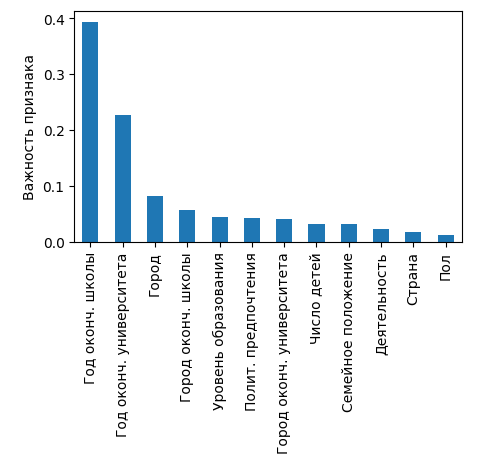
\includegraphics[width=\linewidth]{images/rf_age_feature_importance}
\caption{Возраст}
\end{subfigure}
\hfill
\begin{subfigure}[h]{0.5\linewidth}
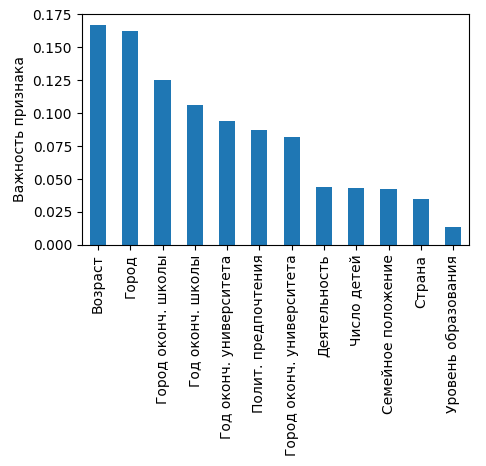
\includegraphics[width=\linewidth]{images/rf_gender_feature_importance.png}
\caption{Пол}
\end{subfigure}%
\caption{Оценка важности признаков случайного леса в задачах определения возраста и пола}
\label{fig:rf_feature_importace}
\end{figure}



\subsection{2.8. Градиентный бустинг}

Градиентный бустинг \cite{gradient boosting} -- это техника машинного обучения для задач классификации и регрессии, которая строит модель в форме ансамбля слабых предсказывающих моделей, обычно деревьев решений. Главное отличие от случайного леса заключается в том, что в бустинге базовые модели строятся последовательно и каждый следующий алгоритм строится таким образом, чтобы исправить ошибки уже построенной композиции.

Данный метод имеет как преимущества, так и недостатки. Во-первых, главным плюсом является рассмотрение любого семейства базовых алгоритмов. А это дает широкие возможности для учета особенностей исходной задачи. Как правило, бустинг над решающими деревьями считается одним из эффективных вариантов использования данной модели. Помимо этого, данный алгоритм является довольно простым и имеет четкое математическое обоснование, что позволяет в каждой конкретной вариации бустинга сделать некоторые математические и алгоритмические оптимизации, которые могут ускорить работу алгоритма.

\setlength\extrarowheight{8pt}
\begin{table}[h!]
\centering
\begin{tabular}{|c|l|}
\hline
\textbf{Выборка}            & Исходная \\ \hline
\textbf{MAE}                & 2.29  \\ \hline
\textbf{Число деревьев}      & 1473     \\ \hline
\textbf{Максимальная глубина дерева}         & 3        \\ \hline
\textbf{L1 регуляризация}         & 138.94   \\ \hline
\textbf{L2 регуляризация}        & 0.0167   \\ \hline
\end{tabular}
\caption{Результаты градиентного бустинга для определения возраста}
\label{gradient boosting age table}
\end{table}

Что касается недостатков, то  как правило бустинг работает достаточно медленно, поскольку требуется построение сотен или даже тысяч базовых методов, которые входят в композицию. Также, данный метод имеет свойство очень сильно подстраиваться под данные, в том числе под выбросы в данных, что ведет в свою очередь к переобучению. И, наконец, результаты работы бустинга довольно сложно интерпретировать, особенно
если в композицию входят десятки алгоритмов.  Помимо этого, поскольку каждый последующий базовый алгоритм пытается исправить ошибки предыдущего, то гралиентный бустинг в целом сложно распараллелить.




\begin{table}[t]
\centering
\begin{tabular}{|c|l|}
\hline
\textbf{Выборка}            & Исходная \\ \hline
\textbf{Accuracy}           & 0.715    \\ \hline
\textbf{Precision}          & 0.636    \\ \hline
\textbf{Recall}             & 0.222    \\ \hline
\textbf{F1}                 & 0.329   \\ \hline
\textbf{Число деревьев}      & 4314     \\ \hline
\textbf{Максимальная глубина дерева}         & 3        \\ \hline
\textbf{L1 регуляризация}         & 0.022    \\ \hline
\textbf{L2 регуляризация}        & 1.0      \\ \hline
\end{tabular}
\caption{Результаты градиентного бустинга для определения пола}
\label{gradient boosting gender table}
\end{table}


\begin{figure}[h!]
\begin{subfigure}[h]{0.5\linewidth}
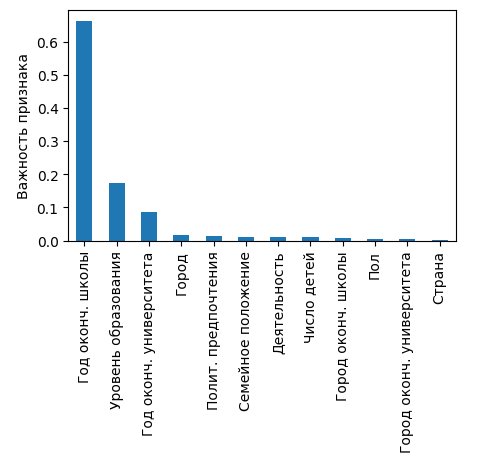
\includegraphics[width=\linewidth]{images/xgb_age_feature_importance}
\caption{Возраст}
\end{subfigure}
\hfill
\begin{subfigure}[h]{0.5\linewidth}
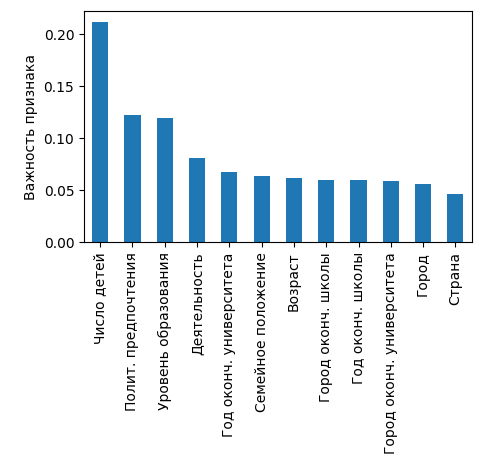
\includegraphics[width=\linewidth]{images/xgb_gender_feature_importance.png}
\caption{Пол}
\end{subfigure}%
\caption{Оценка важности признаков градиентного бустинга в задачах определения возраста и пола}
\label{fig:xgb_feature_importace}
\end{figure}

Для решения поставленных задача, а именно определение возраста и пола пользователя используется библиотека XGBoost \cite{xgboost}, которая является одной из самых популярных и эффективных реализаций градиентного бустинга на решающих деревьях. Подбор параметров выполнен с помощью кросс-валидации тренировочного множества. Полученные результаты можно наблюдать в Таблице \ref{gradient boosting age table} и в Таблице \ref{gradient boosting gender table}.


Графики оценки важности признаков представлены на Рис. \ref{fig:xgb_feature_importace}. В отличие от случайного леса, помимо года окончания школы для градиентного бустинга имеет значение также уровень образования пользователя для определения возраста, а для определения пола -- число детей, политические взгляды и уровеь образования.




\clearpage






